\section{Experimental results} \label{experimental_results}

% TODO: The third section shall report experimental results (e.g. training progress diagrams), describe interesting observations, and discuss the difficulties you faced and how you overcame them.

When starting the initial training process first a pre-training is executed which serves to fill the prioritized experience replay buffer with experiences from an expert rule-based agent and to pre-train the model itself to build up on some agent behavior already for the later training process. To not introduce a heavy bias the pre-training is stopped after 1.500 training games. \autoref{fig:pre-loss-1} shows the aggregated step loss per episode averaged after five episodes and \autoref{fig:pre-reward-1} the reward per episode averaged after five episodes.

\begin{figure}[ht]
	\centering
	\begin{subfigure}[b]{0.49\textwidth}
		\centering
		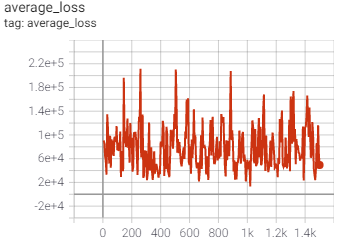
\includegraphics[width=\textwidth]{figures/training1-pre-loss.PNG}
		\caption{Pre-training loss}
		\label{fig:pre-loss-1}
	\end{subfigure}
	\hfill
	\begin{subfigure}[b]{0.49\textwidth}
		\centering
		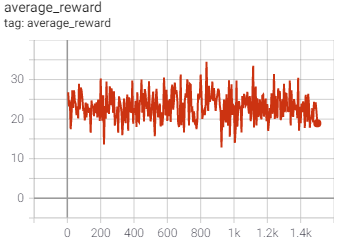
\includegraphics[width=\textwidth]{figures/training1-pre-reward.PNG}
		\caption{Pre-training average reward}
		\label{fig:pre-reward-1}
	\end{subfigure}
\end{figure}

The two charts are not too surprising, the reward should on average be the same with a rule-based behavior. Also the loss does not decrease much with only 1.500 episodes of pre-training. When initiating the main training process with experiences gained from the dueling double DQN itself the following training curves can be experienced:

\begin{figure}[ht]
	\centering
	\begin{subfigure}[b]{0.49\textwidth}
		\centering
		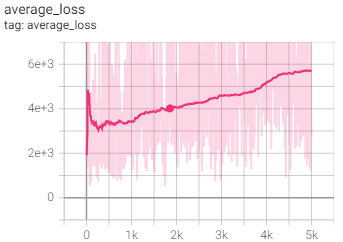
\includegraphics[width=\textwidth]{figures/training1-main-loss-smooth.PNG}
		\caption{Main-training loss}
		\label{fig:main-loss-smoothed-1}
	\end{subfigure}
	\hfill
	\begin{subfigure}[b]{0.49\textwidth}
		\centering
		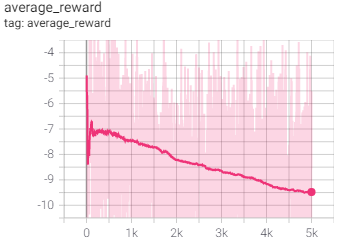
\includegraphics[width=\textwidth]{figures/training1-main-reward-smooth.PNG}
		\caption{Main-training average reward}
		\label{fig:main-reward-smoothed-1}
	\end{subfigure}
\end{figure}

The complete opposite of what was expected was observed, the loss increased whereas the average reward decreased. One possible explanation was a possible training bias introduced through the prioritized experience replay buffer towards transition with a high temporal difference error. Even if the gradient weighting factors were calculated and used to anneal the bias as proposed in the original paper, still this unintended behavior could be experienced. Therefore the training process was aborted after 5.000 episodes. 

The next generation of the model was trained on a normal experience replay buffer with the following results:

\begin{figure}[ht]
	\centering
	\begin{subfigure}[b]{0.49\textwidth}
		\centering
		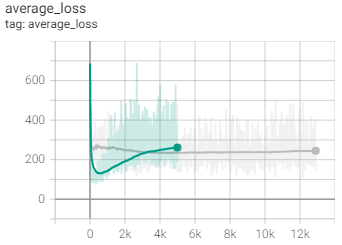
\includegraphics[width=\textwidth]{figures/training2-main-loss-smooth.PNG}
		\caption{Main-training loss}
		\label{fig:main-loss-smoothed-2}
	\end{subfigure}
	\hfill
	\begin{subfigure}[b]{0.49\textwidth}
		\centering
		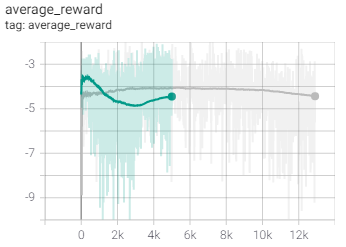
\includegraphics[width=\textwidth]{figures/training2-main-reward-smooth.PNG}
		\caption{Main-training average reward}
		\label{fig:main-reward-smoothed-2}
	\end{subfigure}
\end{figure}

Also, the initial exploration factor $\epsilon$ was increased from 0.3 to 1 to counter a possible pre-training bias and the maximum size of the experience replay buffer was decreased from 65.536 to 32.768 to train on more recent experiences. The green curve shows the training development until 5.000 episodes, which was then expanded to another 13.000 episodes plotted in the gray curve. 

Having done these changes results in a far lower training loss curve which converges to an average episode loss of 250 per five episodes. Also the reward curve seems to converge at an average loss of about minus four. Nevertheless, this average reward still is not what was expected and when looking at the actual agent behavior, the agent always chooses to wait. A possible explanation for this might be that the agent tries to avoid future punishments by just waiting until it gets killed by another player. 

To escape the bad local optimum and the small degree between rewards and punishments, the reward function was first slightly adjusted by increasing the magnitue of each reward by 100 and therefore breaking the normalization. This results in the two following training curves:

\newpage

\begin{figure}[ht]
	\centering
	\begin{subfigure}[b]{0.49\textwidth}
		\centering
		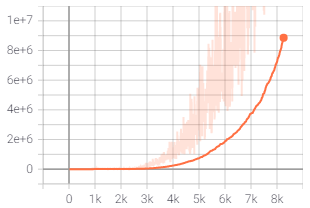
\includegraphics[width=\textwidth]{figures/training3-main-loss-smooth.PNG}
		\caption{Main-training loss}
		\label{fig:main-loss-smoothed-3}
	\end{subfigure}
	\hfill
	\begin{subfigure}[b]{0.49\textwidth}
		\centering
		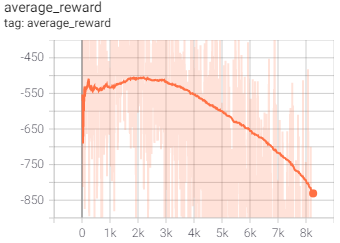
\includegraphics[width=\textwidth]{figures/training3-main-reward-smooth.PNG}
		\caption{Main-training average reward}
		\label{fig:main-reward-smoothed-3}
	\end{subfigure}
\end{figure}

As one can see this negatively impacts the training behavior exponentially and got discarded right away. In the next try the adaption of the rewards were discarded again, the exploration factor $\epsilon$ remained at a start value of one and the maximum size of the experience replay buffer was left at 32.768. The amount of episodes to train during the main training was increased to 30.000. This equals three generations which should show at least some improvements during the training process as in \cite{Kormelink2018} (see \autoref{fig:exploration}), especially when increasing the exploration. The following training curves were experienced: 

\begin{figure}[ht]
	\centering
	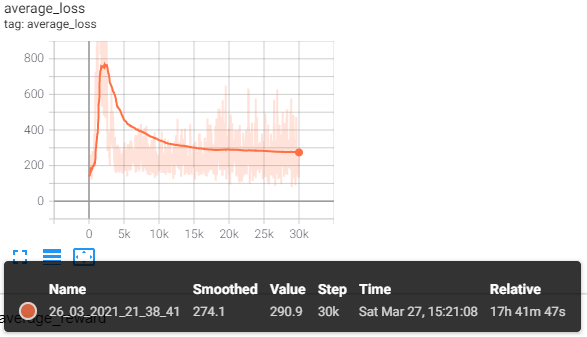
\includegraphics[width=0.8\textwidth]{figures/training4-main-loss-smooth.PNG}
	\caption{Main-training loss}
	\label{fig:main-loss-smoothed-4}
\end{figure}

When looking at the smoothed loss (see \autoref{fig:main-loss-smoothed-4}) one can see the curve falls strictly monotonously from 1.155 after around 2.000 episodes to 291 after 30.000 episodes. Having this setup taking the loss to around zero would still take ages when training locally. One could increase the learning rate, but previous experiments showed that this highly destabilized the training as the learning rate with 0.01 is already quite high compared to other papers \cite{Franca2019, Kormelink2018}. 

\begin{figure}[ht]
	\centering
	\begin{subfigure}[b]{0.49\textwidth}
		\centering
		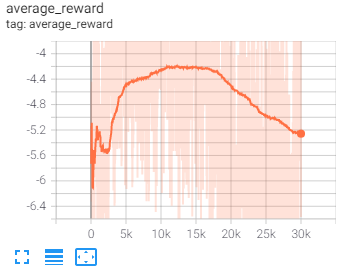
\includegraphics[width=\textwidth]{figures/training4-main-reward-smooth.PNG}
		\caption{Main-training average reward}
		\label{fig:main-reward-smoothed-4}
	\end{subfigure}
	\hfill
	\begin{subfigure}[b]{0.49\textwidth}
		\centering
		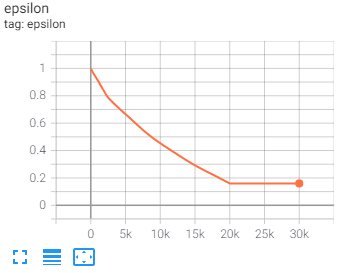
\includegraphics[width=\textwidth]{figures/training4-epsilon.PNG}
		\caption{$\epsilon$-decay}
		\label{fig:epsilon-4}
	\end{subfigure}
\end{figure}

Having higher exploration did not fix the problem of ecaping the bad local optimum of the agent waiting until it gets killed. Instead it just seems to extend the training process as the loss is even higher than before. The course of the average reward curve (see \autoref{fig:main-reward-smoothed-4}) equals to the original one, but now after 18k episodes the average reward curve falls again. This development also seems to be independent from the exploration rate development (see \autoref{fig:epsilon-4}) that now reaches its lower bound far later after 20.000 episodes. 

To summarize neither changing the magnitude of the rewards, nor increasing the exploration rate helped to escape the bad local optimum. Only increasing the training episodes seems to very slowly decrease the loss which might result in another optimum in the future as one would expect when looking at \autoref{fig:exploration}. The 30.000 episode training mark was reached after 17,67 hours which means another approx. 41 hour training to reach the 10 generations mark. As such a training takes its time and does not guarantee its success, it was decided to not pursue this further in the given amount of time. 


